\chapter{Soil modules}

\section{Water balance modules}

Plant growth involves intake of atmospheric CO$_{{\rm 2}}$ through stomatal openings in the
epidermis. Most of the water that plants take up from the soil is again lost to the
atmosphere by transpiration through the same openings. The daily turnover can be
considerable: transpiration from 0.4 cm of water from a crop surface on a clear sunny
day corresponds with a water loss from the root zone of than 40.000 kg ha$^{{\rm -1}}$ 
d$^{{\rm -1}}$. If soil
moisture take up by the roots is not replenished, the soil will dry out to such an extent
that the plants wilt and - ultimately - die.

The tenacity with which the soil retains its water is equalled by the suction which the
roots must exert to be able to take up soil moisture. This suction known as the soil
moisture potential or 'matric suction', can be measured. In hydrology, the potential is
usually used and is expressed as energy unit per weight of soil water, with the dimension
of length (van Bakel, 1981). An optimum range exists within which the plant takes up
water freely. Above or below this level the plant senses stress. It reacts by actively
curbing its daily water consumption through partial or complete closure of the stomata.
The consequence is evident: this stomatal closure interferes with CO$_{{\rm 2}}$ intake and 
reduces assimilation and, consequently, dry matter production.

A crop growth simulation model must therefore keep track of the soil moisture potential
to determine when and to what degree a crop is exposed to water stress. This is commonly 
done with the aid of a water balance equation, which compares for a given period of
time, incoming water in the rooted soil with outgoing water and quantifies the difference
between the two as a change in the amount of soil moisture stored.

Therefore the purpose of the soil water balance calculations is to estimate the daily value
of the actual soil moisture content, which influences soil moisture uptake and crop
transpiration.

\begin{figure}[p]
	%Fig. 6.1
	\centering
	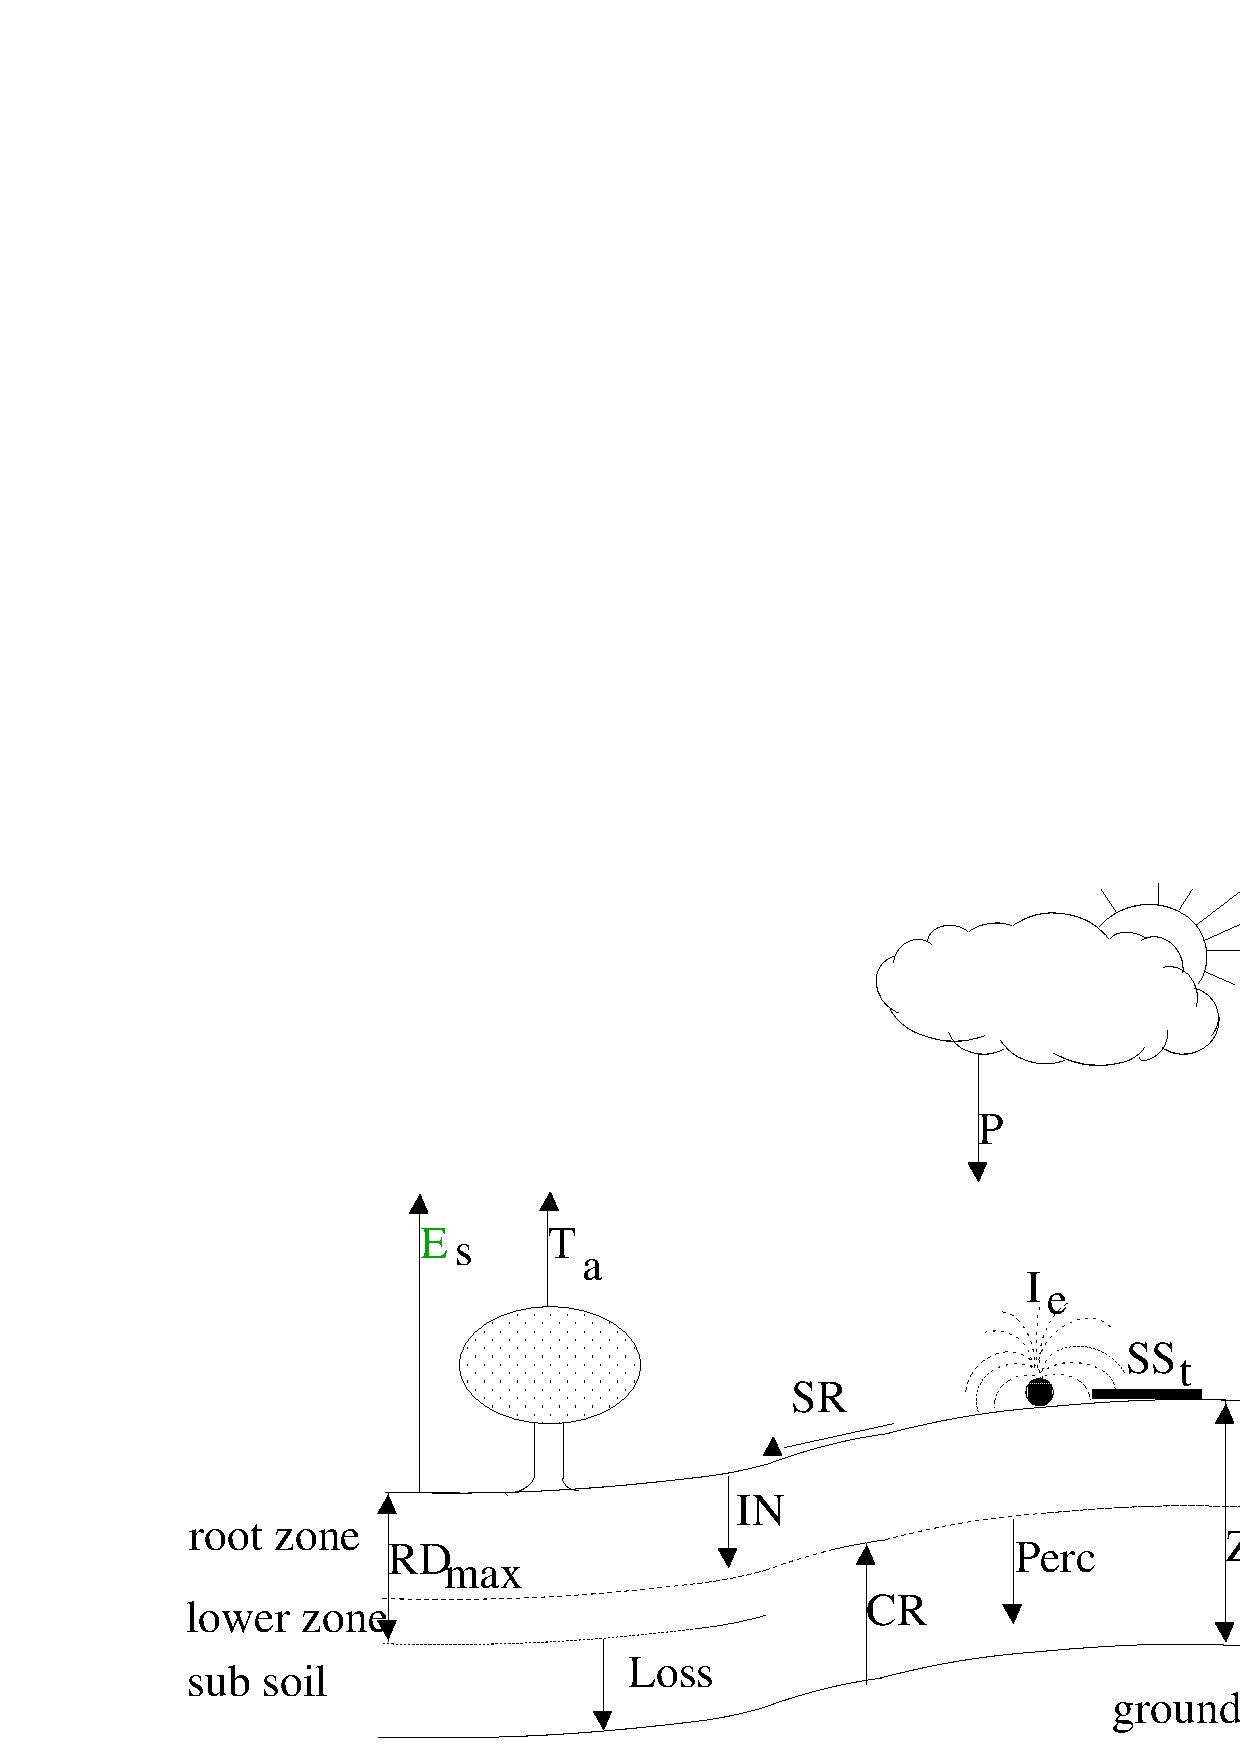
\includegraphics[width=120mm]{\FigDir/WATBAL1.pdf}
	\caption{Schematic representation of the different components of a soil water balance}
	\label{fig:WatBalSchematic}
\end{figure}

The actual soil moisture content can be established according to (Driessen, 1986):

\stepcounter{equation}
\begin{align}
% equations 6.1a-b
\label{eq:6.1}
\theta_{t~} &= {\frac{IN _{up} ~+~(IN _{low} ~-~T _{a} )}{RD}} \Delta t \subeqn \\[1em]
IN_{up} &= P~+~I _{e} ~-~E _{s} ~+~SS _{t} \, /\Delta t-~SR  \subeqn  \\[1em]
IN_{low} &= CR~-~Perc \subeqn
\end{align}

Where:\\[5pt]
\begin{tabularx}{\textwidth}{llXr}
	$\theta$$_{{\rm t}}$ &:& Actual moisture content of the root zone at time step t
	& [cm$^{{\rm 3}}$ cm$^{{\rm -3}}$]\\
	IN$_{{\rm up}}$ &:& Rate of net influx through the upper root zone boundary
	& [cm d$^{{\rm -1}}$]\\
	IN$_{{\rm lo}}$$_{{\rm w}}$ &:& Rate of net influx through the lower root zone boundary
	& [cm d$^{{\rm -1}}$]\\
	T$_{{\rm a}}$ &:& Actual transpiration rate of crop
	& [cm d$^{{\rm -1}}$]\\
	RD &:& Actual rooting depth  & [cm]\\
	P &:& Precipitation intensity  & [cm d$^{{\rm -1}}$]\\
	I$_{{\rm e}}$ &:& Effective daily irrigation  & [cm d$^{{\rm -1}}$]\\
	E$_{{\rm s}}$ &:& Soil evaporation rate   & [cm d$^{{\rm -1}}$]\\
	SS$_{{\rm t}}$ &:& Surface storage  & [cm]\\
	SR &:& Rate of surface runoff  & [cm d$^{{\rm -1}}$]\\
	CR &:& Rate of capillary rise  & [cm d$^{{\rm -1}}$]\\
	Perc &:& Percolation rate  & [cm d$^{{\rm -1}}$]\\
	$\Delta$t &:& Time step  & [d]\\
	Z$_{{\rm t}}$ &:& Depth of groundwater table (see figure \ref{fig:WatBalSchematic})  & [cm]\\
\end{tabularx}

Processes directly affecting soil moisture content of the root zone can be defined as:
\begin{itemize}
	\item infiltration is transport from the soil surface into the root zone;
	\item evaporation is the loss of soil moisture to the atmosphere through the soil surface;
	\item transpiration by plants is loss of soil moisture to the atmosphere 
	      from the entire root zone;
	\item percolation is downward transport of water from the root zone to the layer below the root zone;
	\item capillary rise is upward transport into the rooted zone.
\end{itemize}

The water balance equation has to be solved for each time interval in the crop growth cycle.

For the calculation of potential production the soil moisture content is
assumed to be at field capacity and no calculations have to be performed to simulate the
water balance in the soil. Only the crop water requirements are quantified as the sum of 
crop transpiration and evaporation from the shaded soil under the canopy. 

For the calculation of the water limited production three different soil water balances are
distinguished. The first water balance (called \emph{Classic water balance}) applies to a freely draining soil, where groundwater is so deep that it cannot have influence on the soil moisture content in the rooting zone. The soil profile is divided in two compartments, the rooted zone and the lower zone between actual rooting depth and maximum rooting depth. The subsoil below the maximum rooting depth is not defined. The second zone merges gradually with the first zone as the roots grow deeper towards the maximum rooting depth. This water balance applies to (regional) applications with limited information on soil properties.

The second water balance (called \emph{Layered water balance}) takes into account the impact of different soil layers and the influence of groundwater. This water balance uses a simple but elegant solution to estimate water flow through the soil taking into account both gravitational flow as well flow due to differences in matric suction and groundwater. It is targeted at making good estimates of crop water availability under conditions when properties of the soil are well known, but without going into the complexity of Richard's equation type of soil water models. 

Finally, the WOFOST implementation connected to the SWAP model has a detailed water balance which including multiple soil layers and variable integration time steps to account for highly non-linear processes in the soil. Besides estimating water availability, SWAP also deals with soil temperature and solute transport which allows to make 
detailed simulations of the behaviour of water and solutes in the soil and its impact on plant growth.
The SWAP water balance is not treated in this manual as SWAP has its own set of documentation 
\footnote{http://www.swap.alterra.nl} where the theory and usage of the model is described.

\subsection{The classic Water balance}
\label{sec:WATFD}

For the rooted zone the water balance equation is solved every daily time step. At the
upper boundary, processes comprise the infiltration of water from precipitation or
irrigation, evaporation from the soil surface and uptake of water and transpiration by the
crop. If rainfall intensity exceeds the infiltration and surface storage capacity of the soil,
water runs off. Water can be stored in the soil till the field capacity is reached. Additional
water percolates beyond the lower boundary of the rooting zone.
The flow rates are limited by the maximum percolation rate of the root zone and the
maximum percolation rate of the water to the subsoil.

The textural profile of the soil is conceived homogeneous. Initially the soil profile
consists of three layers (zones):
\begin{itemize}
	\item the rooted zone between soil surface and actual rooting depth
	\item the lower zone between actual rooting depth and maximum rooting depth
	\item the subsoil below maximum rooting depth
\end{itemize}

The extension of the root zone from initial rooting depth to maximum rooting depth is
described in \S \ref{sec:rootgrowth}. Its effect on the soil moisture content is accounted 
for in this soil water
balance calculation. From the moment that the maximum rooting depth is reached the soil
profile is described as a two layer system (Driessen, 1986). The lower zone no longer
exists.

The water balance is driven by rainfall, possibly buffered as surface storage, and
evapotranspiration. The processes considered are infiltration, soil water retention,
percolation and the loss of water beyond the maximum root zone.

As mentioned earlier, no groundwater influence is assumed, therefore capillary rise is not
accounted for. Only downward flow, evaporation from the soil surface and transpiration
are included in the calculations. 

\subsubsection{Initial soil water content and initial soil water amount}

The initial value of the actual soil moisture content in the rooted part of the soil can be
calculated as:

\begin{equation}
\label{eq:6.18}
\theta_{t} ~ =~\theta_{wp} ~+~{\frac{W_{av}}{RD}}
\end{equation}

Where:\\[5pt]
\begin{tabularx}{\textwidth}{llXr}
	$\theta$$_{{\rm t}}$ &:& Actual soil moisture content in rooted z
	one  & [cm$^{{\rm 3}}$ cm$^{{\rm -3}}$]\\
	$\theta$$_{{\rm wp}}$ &:& Soil moisture content at wilting   & [cm$^{{\rm 3}}$ cm$^{{\rm -3}}$]\\
	W$_{{\rm av}}$ &:& Initial amount of available soil moisture 
	in excess of $\theta$$_{{\rm wp}}$ & [cm]\\
	RD &:& Actual rooting depth (see \S 5.5) & [cm]\\
\end{tabularx}

It should be mentioned that the initial actual soil moisture content, $\theta$$_{{\rm t}}$, cannot be lower
than the soil moisture content at wilting point. In case the crop cannot develop airducts,
the initial soil moisture content cannot be higher than the soil moisture content at field
capacity. If the crop can develop airducts the initial soil moisture content cannot exceed
the soil porosity. {\bf W$_{{\rm av}}$} (acronym: {\bf WAV}), the initial amount of available 
soil moisture in excess of $\theta$$_{{\rm wp}}$ should be provided by the user. 

Multiplying the actual soil moisture content with the rooting depth yields the initial
amount of water in the rooted zone. The initial amount of soil moisture in the lower zone,
the zone between the rooted zone and the maximum rooting depth, can be calculated as:

\begin{equation}
\label{eq:6.19}
W_{lz} ~ =~ W _{av} ~+~ RD_{\max } ~\theta_{wp} ~-~RD~\theta_{t} 
\end{equation}

Where:\\[5pt]
\begin{tabularx}{\textwidth}{llXr}
	W$_{{\rm lz}}$ &:& Amount of soil moisture in the lower zone & [cm]\\
	W$_{{\rm av}}$ &:& Initial amount of available soil moisture 
	in excess of $\theta$$_{{\rm wp}}$ & [cm]\\
	RD$_{{\rm max}}$ &:& Maximum rooting depth & [cm]\\
	RD &:& Actual rooting depth & [cm]\\
	$\theta$$_{{\rm t}}$ &:& Actual soil moisture content in rooted zone  
	& [cm$^{{\rm 3}}$ cm$^{{\rm -3}}$]\\
	$\theta$$_{{\rm wp}}$ &:& Soil moisture content at wilting point  
	& [cm$^{{\rm 3}}$ cm$^{{\rm -3}}$]\\
\end{tabularx}

The soil moisture content of the lower zone is also limited by the field capacity in case
the crop cannot develop airducts, else the soil moisture content is limited by the soil
porosity. In the model, initially, the variable D$_{{\rm slr}}$, days since last rain, is set 
to one. If the
actual soil moisture content is halfway between the field capacity and wilting point a
value of five days is assumed. 

\subsubsection{Evaporation}
The evaporation depends on the amount of available water in the soil and the infiltration
capacity of the soil. If the water layer on the surface, the so called surface storage, 
exceeds 1 cm, the actual evaporation rate from the soil is set to zero and the actual
evaporation rate from the surface water is equal to the maximum evaporation from a
shaded water surface.

If the surface storage is less than 1 cm and the infiltration rate of the previous day
exceeds 1 cm d$^{{\rm -1}}$, the actual evaporation rate from the surface water is set to zero and the
actual evaporation rate from the soil is equal to the maximum evaporation from a shaded
soil surface. All water on the surface can infiltrate within one day. The value of the
variable days since last rain, D$_{{\rm slr}}$, is reset to unity.

If the infiltration rate is less than 1 cm d$^{{\rm -1}}$, the amount of infiltrated water is considered
too small to justify a reset of the parameter D$_{{\rm slr}}$ and the evaporation rate decreases as the
top soil starts drying. The reduction of the evaporation is thought to be proportional to the
square root of time (Stroosnijder, 1987, 1982). The evaporation can be calculated as:

\begin{equation}
\label{eq:6.20}
E _{s} ~=~ E _{s,\max } ( \sqrt{D _{slr} } ~-~ \sqrt{D _{slr} \, -\, 1} )
\end{equation}

Where:\\[5pt]
\begin{tabularx}{\textwidth}{llXr}
	E$_{{\rm s}}$ &:& Evaporation rate from a shaded soil surface  & [cm d$^{{\rm -1}}$]\\
	E$_{{\rm s,max}}$ &:& Maximum evaporation rate from a shaded soil
	surface (see eq. \ref{eq:6.7})  & [cm d$^{{\rm -1}}$]\\
	D$_{{\rm slr}}$ &:& Days since last rain  & [d]\\
\end{tabularx}

When a small amount of water has infiltrated, or rather wetted the soil surface, this
amount can be evaporated the same day, irrespective of D$_{{\rm slr}}$. Therefore, the actual
evaporation from the soil surface, as calculated according to equation \ref{eq:6.20}, should be
corrected for this amount of water infiltrating the soil. This amount should be added to
the actual evaporation rate. However, it should be noted that the actual evaporation never
can exceed the maximum evaporation rate.

\subsubsection{Precipitation}
Not all the precipitation will reach the surface. A fraction will be intercepted by leaves,
stems, etc. From the amount of precipitation which reaches the soil surface, not all will
infiltrate. A part runs off. Runoff from a field can be 0-20 percent, and even higher on
unfavorable surfaces (Stroosnijder \& Kon\'{e}, 1982). In the model, it is assumed that a
fixed fraction of the precipitation will not infiltrate on the same day. This fraction can be
reduced in situations with relatively small amounts of rainfall. In the model a reduction
factor is defined as function of the amount of rainfall (van Diepen {\it et al}., 1988). See 
figure \ref{fig:NonInfiltFrac} and equation \ref{eq:6.26}. Note that the non infiltrating 
fraction refers to rainfall only.
Irrigation water is assumed to infiltrate freely. However, the irrigation option is not
implemented in WOFOST 6.0.

\begin{figure}[p]
	% Fig. 6.2 
	\centering
	
\includegraphics[width=110mm]{\FigDir/RED.pdf}
	\caption{Reduction factor of the non infiltrating fraction as a function of rainfall.}
	\label{fig:NonInfiltFrac}
\end{figure}

\subsubsection{Percolation}
If the soil moisture content of the root zone is above field capacity, water percolates to
the lower part of the potentially rootable zone and to the subsoil. In the model, a clear
distinction is made between percolation from the actual rootzone to the so-called lower
zone, and percolation from the lower zone to the subsoil. The former is called Perc and
the latter is called Loss. The percolation rate from the rooted zone can be calculated as:

\begin{equation}
\label{eq:6.21}
Perc  ~=~{\frac{W _{rz} \, -\, W _{rz,\, fc} }{\Delta t}} ~-~ T _{a} ~-~ E _{s} 
\end{equation}

Where:\\[5pt]
\begin{tabularx}{\textwidth}{llXr}
	Perc &:& Percolation rate from the root zone to the lower zone  & [cm d$^{{\rm -1}}$]\\
	W$_{{\rm rz}}$ &:& Amount of soil moisture in the root zone (see eq. \ref{eq:6.33}a)  & [cm]\\
	W$_{{\rm rz,fc}}$ &:& Equilibrium amount of soil moisture in the root
	zone (see eq. \ref{eq:6.22})  & [cm]\\
	$\Delta$t &:& Time step  & [d]\\
	T$_{{\rm a}}$ &:& Actual transpiration rate (see eq. \ref{eq:6.14})  & [cm d$^{{\rm -1}}$]\\
	E$_{{\rm s}}$ &:& Evaporation rate from a shaded soil surface 
	(see eq. \ref{eq:6.7}  and \ref{eq:6.20})  & [cm d$^{{\rm -1}}$]\\
\end{tabularx}

The equilibrium amount of soil moisture in the root zone can be calculated as the soil
moisture content at field capacity times the depth of the rooting zone:

\begin{equation}
\label{eq:6.22}
W _{rz,\, fc} ~=~ \theta  _{fc} \,\, RD
\end{equation}

Where:\\[5pt]
\begin{tabularx}{\textwidth}{llXr}
	W$_{{\rm rz,fc}}$ &:& Equilibrium amount of soil moisture in the root zone  & [cm]\\
	$\theta$$_{{\rm fc}}$ &:& Soil moisture content at field capacity  & 
	[cm$^{{\rm 3}}$ cm$^{{\rm -3}}$]\\
	RD &:& Actual rooting depth  & [cm]\\
\end{tabularx}

The percolation rate is limited by the conductivity of the wet soil (acronym: {\bf SOPE}) in the
same way as the infiltration is limited. The conductivity is soil specific and should be
given by the user. Note that the percolation from the root zone to the lower zone can be
limited by the up take capacity of the lower zone. Therefore, the value calculated with 
equation \ref{eq:6.21} is preliminary. The capacity should first be checked.

The percolation from the lower zone to the subsoil, the so-called Loss, should take the
amount of water in the lower zone into account. If the amount of water in the lower zone
is less than the equilibrium amount of soil moisture, a part of the percolating water will
be retained and the percolation rate will be reduced. The loss of water from the lower end
of the maximum root zone can be calculated as:

\begin{equation}
\label{eq:6.23}
Loss ~=~{\frac{W _{lz} \, -\, W _{lz,\, fc} }{\Delta t}} ~+~ Perc
\end{equation}

Where:\\[5pt]
\begin{tabularx}{\textwidth}{llXr}
	Loss &:& Percolation rate from the lower zone to the subsoil   & [cm d$^{{\rm -1}}$]\\
	Perc &:& Percolation rate from root zone to lower zone (see eq. \ref{eq:6.21})  & [cm d$^{{\rm -1}}$]\\
	W$_{{\rm lz}}$ &:& Amount of soil moisture in the lower zone (see eq. \ref{eq:6.33}b)  & [cm]\\
	W$_{{\rm lz,fc}}$ &:& Equilibrium amount of soil moisture in the
	lower zone (see eq. \ref{eq:6.24})  & [cm]\\
	$\Delta$t &:& Time step   & [d]\\
\end{tabularx}

The loss of water from the potentially rootable zone, is also limited by the maximum
percolation rate of the subsoil. This maximum percolation rate (acronym: {\bf KSUB}) is soil
specific and should be provided by the user. The equilibrium amount of soil moisture in
the lower zone can be calculated as the soil moisture content at field capacity times the
depth of the root zone:

\begin{equation}
\label{eq:6.24}
W_{lz,\, fc} = \theta_{fc} \,\, (RD_{\max} ~-~RD)
\end{equation}

Where:\\[5pt]
\begin{tabularx}{\textwidth}{llXr}
	W$_{{\rm rz,fc}}$ &:& Equilibrium amount of soil moisture in the lower zone  & [cm]\\
	$\theta$$_{{\rm fc}}$ &:& Soil moisture content at field capacity  & [cm$^{{\rm 3}}$ cm$^{{\rm -3}}$]\\
	RD$_{{\rm max}}$ &:& Maximum rooting depth  & [cm]\\
	RD &:& Actual rooting depth  & [cm]\\
\end{tabularx}

For rice an additional limit of five percent of the saturated soil conductivity is set to
account for the effect of puddling (a rather arbitrary value, which may be easily changed
in the program). The saturated soil conductivity (acronym: {\bf K0}) is soil specific. In the
model, K0 is calculated using equating \ref{eq:6.67} with pF= -1.0 (i.e. a hydraulic head of 0.1
cm) The percolation rate from the lower zone to the sub soil is not to exceed this value
(van Diepen {\it et al}., 1988). 

As mentioned before, the value calculated with equation \ref{eq:6.21}, should be regarded as
preliminary. The storage capacity of the receiving layer may become limiting. The
storage capacity of the lower zone, also called the uptake capacity, is the amount of air
plus the loss (van Diepen {\it et al}., 1988). The storage capacity can de defined as:

\begin{equation}
\label{eq:6.25}
UP  ~=~{\frac{(\, RD _{\max } \, -\, RD\, )\, \theta  _{\max } ~-~ W _{lz} }{\Delta t}} ~+~ Loss
\end{equation}

Where:\\[5pt]
\begin{tabularx}{\textwidth}{llXr}
	UP &:& Uptake capacity of lower zone  & [cm d$^{{\rm -1}}$]\\
	RD$_{{\rm max}}$ &:& Maximum rooting depth  & [cm]\\
	RD &:& Actual rooting depth  & [cm]\\
	W$_{{\rm lz}}$ &:& Amount of soil moisture in lower zone  & [cm]\\
	$\theta$$_{{\rm max}}$ &:& Soil porosity (maximum soil moisture)  & [cm$^{{\rm 3}}$ cm$^{{\rm -3}}$]\\
	$\Delta$t &:& Time step  & [d]\\
	Loss &:& Percolation rate from the lower zone to the subsoil   & [cm d$^{{\rm -1}}$]\\
\end{tabularx}

The percolation to the lower part of the potentially rootable zone can not exceed the
uptake capacity of the lower zone. Therefore the percolation rate is equal to the minimum
of the calculated percolation rate (eq. \ref{eq:6.21}) and the uptake.

\subsubsection{Preliminary infiltration}
The infiltration rate depends on the amount of available water and the infiltration capacity
of the soil. If the actual surface storage is less then or equal to 0.1 cm, the preliminary
infiltration capacity is simply described as:

\begin{equation}
\label{eq:6.26}
IN_{p} =~ (\, 1\, -\, F _{I} \, C _{I} \, )\, P~+~ I _{e~} +~ SS _{\frac{t}{ \Delta t}} 
\end{equation}

Where:\\[5pt]
\begin{tabularx}{\textwidth}{llXr}
	IN$_{{\rm p}}$ &:& Preliminary infiltration rate  & [cm d$^{{\rm -1}}$]\\
	F$_{{\rm I}}$ &:& Maximum fraction of rain not infiltrating during time step t  & [-]\\
	C$_{{\rm I}}$ &:& Reduction factor applied to F$_{{\rm I}}$ as a function of the 
	precipitation intensity  & [-]\\
	P &:& Precipitation intensity  & [cm d$^{{\rm -1}}$]\\
	I$_{{\rm e}}$ &:& Effective irrigation  & [cm d$^{{\rm -1}}$]\\
	SS$_{{\rm t}}$ &:& Surface storage at time step t (see eq. \ref{eq:6.29})  & [cm]\\
	$\Delta$t &:& Time step  & [d]\\
\end{tabularx}

The maximum fraction of rain not infiltrating during time step t, {\bf F$_{{\rm I}}$} 
(acronym: {\bf NOTINF})
can be either set to a fixed value or be made variable by multiplying F$_{{\rm I}}$ 
with a precipitation dependent reduction factor {\bf C$_{{\rm I}}$} (acronym: {\bf NINFTB}). 
If the fraction is variable, it means that it is maximum for high rainfall amounts, and 
that it will be reduced for low rainfall. The user should provide F$_{{\rm I}}$. 
Values of the C$_{{\rm I}}$ table are included in the model and
are assumed to be fixed. The infiltration rate calculated is preliminary, as the storage
capacity of the soil is not yet taken into account. 

If the actual surface storage is more than 0.1 cm, the available water which can 
potentially infiltrate, is equal to the amount of water, present on the surface, that is supplied via
rainfall and irrigation and depleted via evaporation from the water surface:

\begin{equation}
\label{eq:6.27}
IN_{p} ~=~P~+~I _{e} ~-~ E _{w~} +~ SS _{\frac{t}{\Delta t}} 
\end{equation}

Where:\\[5pt]
\begin{tabularx}{\textwidth}{llXr}
	IN$_{{\rm p}}$ &:& Preliminary infiltration rate  & [cm d$^{{\rm -1}}$]\\
	P &:& Precipitation intensity  & [cm d$^{{\rm -1}}$]\\
	I$_{{\rm e}}$ &:& Effective irrigation  & [cm d$^{{\rm -1}}$]\\
	E$_{{\rm w}}$ &:& Evaporation rate from a shaded water surface  & [cm d$^{{\rm -1}}$]\\
	SS$_{{\rm t}}$ &:& Surface storage at time step t (see eq. 6.29)  & [cm]\\
	$\Delta$t &:& Time step  & [d]\\
\end{tabularx}

However, the infiltration rate is hampered by the conductivity of the soil. The calculated
infiltration rate cannot exceed the conductivity of the soil, which is used as an infiltration
limit. The conductivity of the soil (acronym: {\bf SOPE}) is soil specific and should be given
by the user.

\subsubsection{Adjusted infiltration}
The total loss of water from the root zone can now be calculated as the sum of the
transpiration, the evaporation and the percolation. The sum of this loss and the available
pore space in the root zone define the maximum infiltration rate. The preliminary
infiltration rate cannot exceed this value. The maximum possible infiltration rate is given
by:

\begin{equation}
\label{eq:6.28}
IN_{\max } ~=~{\frac{(\, \theta  _{\max } \, -\, \theta  _{t} \, )\, RD}{\Delta t}} ~+~ T _{a} ~+~ E _{s} ~+~ Perc
\end{equation}

Where:\\[5pt]
\begin{tabularx}{\textwidth}{llXr}
	IN$_{{\rm max}}$ &:& Maximum infiltration rate  & [cm d$^{{\rm -1}}$]\\
	$\theta$$_{{\rm max}}$ &:& Soil porosity (maximum soil moisture)  
	& [cm$^{{\rm 3}}$ cm$^{{\rm -3}}$]\\
	$\theta$$_{{\rm t}}$ &:& Actual soil moisture content  
	& [cm$^{{\rm 3}}$ cm$^{{\rm -3}}$]\\
	RD &:& Actual rooting depth  & [cm]\\
	$\Delta$t &:& Time step  & [d]\\
	T$_{{\rm a}}$ &:& Actual transpiration rate   & [cm d$^{{\rm -1}}$]\\
	E$_{{\rm s}}$ &:& Evaporation rate from a shaded soil surface  & [cm d$^{{\rm -1}}$]\\
	Perc &:& Percolation rate from root zone to lower zone  & [cm d$^{{\rm -1}}$]\\
\end{tabularx}

\subsubsection{Surface runoff}

Surface runoff is also taken into account by defining a maximum value for the surface
storage. If the surface storage exceeds the maximum value for surface storage the
exceeding amount of water will run off. The surface storage at time step t can be
calculated as:

\begin{equation}
\label{eq:6.29}
SS_{t} ~=~ SS _{t-1} ~+~ (\, P ~+~ I _{e} ~-~ E _{w} ~-~ IN\, )\, \Delta t
\end{equation}

Where:\\[5pt]
\begin{tabularx}{\textwidth}{llXr}
	SS$_{{\rm t}}$ &:& Surface storage at time step t  & [cm d$^{{\rm -1}}$]\\
	P &:& Precipitation intensity  & [cm d$^{{\rm -1}}$]\\
	I$_{{\rm e}}$ &:& Effective irrigation rate  & [cm d$^{{\rm -1}}$]\\
	E$_{{\rm w}}$ &:& Evaporation rate from a shaded water surface  & [cm d$^{{\rm -1}}$]\\
	IN &:& Infiltration rate (adjusted)  & [cm d$^{{\rm -1}}$]\\
\end{tabularx}

The surface runoff can be calculated as:

\begin{equation}
%6.30
SR_{t} = SS_{t} - \min (SS_{t}, SS_{\max})\\
\end{equation}

Where:\\[5pt]
\begin{tabularx}{\textwidth}{llXr}
	SR$_{{\rm t}}$ &:& Surface runoff at time step t  & [cm]\\
	SS$_{{\rm t}}$ &:& Surface storage at time step t  & [cm]\\
	SS$_{{\rm max}}$ &:& Maximum surface storage  & [cm]\\
\end{tabularx}

{\bf SS$_{{\rm max}}$} (acronym: {\bf SSMAX}) is an environmental specific variable 
and should be provided by the user.

\subsubsection{Rates of change and root extension}
The rates of change in the amounts of water in the root zone and the lower zone are
calculated straightforward from the flows found above:

\stepcounter{equation}
\begin{align}
\label{eq:6.31}
\Delta W _{rz} &=~ (IN ~-~ T _{a} ~-~ E _{s} ~-~ Perc)\,\Delta \, t  \subeqn  \\
\Delta W _{lz} &=~ (Perc ~-~ Loss)\,\Delta \, t \subeqn
\end{align}

Where:\\[5pt]
\begin{tabularx}{\textwidth}{llXr}
	$\Delta$W$_{{\rm rz}}$ &:& Change of the amount of soil moisture in the root zone  & [cm]\\
	$\Delta$W$_{{\rm lz}}$ &:& Change of the amount of soil moisture in the lower zone  & [cm]\\
	T$_{{\rm a}}$ &:& Actual transpiration rate   & [cm d$^{{\rm -1}}$]\\
	E$_{{\rm s}}$ &:& Evaporation rate from a shaded soil surface  & [cm d$^{{\rm -1}}$]\\
	IN &:& Infiltration rate  & [cm d$^{{\rm -1}}$]\\
	Perc &:& Percolation rate from root zone to lower zone  & [cm d$^{{\rm -1}}$]\\
	Loss &:& Percolation rate from lower zone to sub soil  & [cm d$^{{\rm -1}}$]\\
	$\Delta$t &:& Time step  & [d]\\
\end{tabularx}

Due to extension of the roots into the lower zone, extra soil moisture becomes available.
The amount of the extra soil moisture in the new rootzone and the amount of water in the
reduced lower zone can be calculated as:

\begin{equation}
\label{eq:6.32}
\Delta W _{rz} ~=~\Delta W _{lz} ~=~ W _{lz} \,{\frac{ RD _{t} \, -\, RD _{t-1} }{RD _{\max } \, -\, RD _{t-1} }}
\end{equation}

Where:\\[5pt]
\begin{tabularx}{\textwidth}{llXr}
	RD$_{{\rm t}}$ &:& Rooting depth at time step t  & [cm]\\
	RD$_{{\rm t-1}}$ &:& Rooting depth at time step t-1  & [cm]\\
	RD$_{{\rm max}}$ &:& Maximum rooting depth  & [cm]\\
	W$_{{\rm lz}}$ &:& Amount of soil moisture in the lower zone (see eq. \ref{eq:6.33}b)  & [cm]\\
	$\Delta$W$_{{\rm rz}}$ &:& Change of the amount of soil moisture in the root zone  & [cm]\\
	$\Delta$W$_{{\rm lz}}$ &:& Change of the amount of soil moisture in the lower zone  & [cm]\\
\end{tabularx}

With equation \ref{eq:6.31} the actual amount of water in the root zone and in the lower zone can
be calculated according to:

\stepcounter{equation}
\begin{align}
\label{eq:6.33}
W _{rz,t} ~=~ W _{rz, t-1} ~+~ \Delta W _{rz} \subeqn  \\
W _{lz,t} ~=~ W _{lz, t-1} ~\, +~ \Delta W _{lz} \subeqn
\end{align}

Where:\\[5pt]
\begin{tabularx}{\textwidth}{llXr}
	W$_{{\rm rz,t}}$ &:& Amount of soil moisture in the root zone at time step t  & [cm]\\
	W$_{{\rm lz,t}}$ &:& Amount of soil moisture in the lower zone at time step t  & [cm]\\
	W$_{{\rm rz,t-1}}$ &:& Amount of soil moisture in the root zone at time step t-1  & [cm]\\
	W$_{{\rm lz,t-1}}$ &:& Amount of soil moisture in the lower zone at time step t-1  & [cm]\\
	$\Delta$W$_{{\rm rz}}$ &:& Rate of change of the amount of soil moisture in the root 
	zone  & [cm]\\
	$\Delta$W$_{{\rm lz}}$ &:& Rate of change of the amount of soil moisture in the 
	lower zone  & [cm]\\
\end{tabularx}

\subsubsection{Actual soil moisture content}
The actual soil moisture content can now be calculated according to (see also eq. \ref{eq:6.1}):

\begin{equation}
\label{eq:6.34}
\theta _{t} ~=~ W _{\frac{rz, t}{RD}} 
\end{equation}

Where:\\[5pt]
\begin{tabularx}{\textwidth}{llXr}
	$\theta$$_{{\rm t}}$ &:& Actual soil moisture content at time step t  & [cm$^{{\rm 3}}$ cm$^{{\rm -3}}$]\\
	W$_{{\rm rz,t}}$ &:& Amount of soil moisture in the root zone at time step t  & [cm]\\
	RD &:& Actual rooting depth  & [cm]\\
\end{tabularx}

\subsection{The layered water balance with groundwater influence}

\subsection{The SWAP water balance}

The WOFOST implementation connected to the SWAP model has a detailed water balance which including 
multiple soil layers and variable integration time steps to account for highly non-linear processes 
in the soil. Besides estimating water availability, SWAP also deals with soil temperature and solute 
transport which allows to make 
detailed simulations of the behaviour of water and solutes in the soil and its impact on plant growth.
The SWAP water balance is not treated in this manual as SWAP has its own set of documentation 
\footnote{http://www.swap.alterra.nl} where the theory and usage of the model is described.

\section{The soil nutrient balance for N/P/K}


\section{The SnowMAUS module}

